\documentclass[a4paper]{article}
\usepackage[pdftex]{graphicx}
\usepackage[section]{placeins}

%opening
\title{Prolog Programming Project - Walker}
\author{Andreas Hallberg \\ \texttt{anhallbe@kth.se}}

\begin{document}

\maketitle

\section{Problem}
The program (Walker) finds the shortest path from one point to another in a NxN grid. The paths consist of a number of horizontal and vertical steps (no diagonals). The shortest path through such a grid is always the Manhattan Distance, i.e the sum of the horizontal and vertical distance between two points, so to make the problem more interesting I've added obstacles to the grid. Figure \ref{grid} shows an example of the problem.

\begin{figure}
\centering
	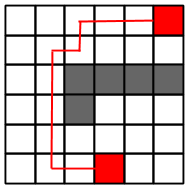
\includegraphics[scale=0.6]{prolog_grid}
	\caption{Example of a grid with 5 obstacles, one of the shortest paths (11 steps) is represented by the red line.}
	\label{grid}
\end{figure}
\FloatBarrier

\section{Solution}
There are many ways to solve the problem. I experimented with two different solutions:
\begin{itemize}
\item{\textbf{Random Walker}} From any given point, walk in a (\textbf{one}) randomly selected direction (Left, Right, Up, Down). Do this until a path has been found from the starting point to the end point. To find the shortest path, simply run the program multiple times and compare the path length for each solution. The advantage of this is that it's possible to quickly find a path without testing every possible step. On the other hand, there is no guarantee that it will find a path at all during one execution, and there is no way to check whether the path is actually the shortest possible.

\item{\textbf{Improved Walker}} From any given point, try walking in \textbf{all} directions. Every combination of steps that takes the walker from the Start point to the End will be a solution. When all solutions are found, their path lengths are compared to find the shortest. The advantage of this strategy is that it is guaranteed to find \textbf{all} paths, including the shortest one. The disadvantages of the strategy is that it will keep looking for other paths even though the shortest has been found, and that the number of possible paths grows exponentially with the size of the grid.
\end{itemize}

\section{The Walker Module}
I implemented both strategies, but I preferred the Improved Walker since it is guaranteed to actually find the shortest path, and finding all possible paths might be of more use when solving other problems.

It exposes one predicate \textit{find(+Start, +End, +Obstacles, +N, -Path, -Steps)}. Start and End are coordinates with the format (X,Y), where  ${Coordinates \in [0,N)}$. Obstacles and Path are list of coordinates, N is the size of the grid and Steps is the length of the resulting shortest Path.

A predicate \textit{walk/6} is used to recursively walk around the grid to look for possible solutions. It is defined as \textit{walk(+Current, +Goal, +Obstacles, +N, +Walked, -Path)}. In short, it is true when Path contains all possible paths from Start to End. It will find the paths by using the walk\_right/6, walk\_left, walk\_up/6 and walk\_down/6 predicates.

\section{Test}
When running the program, it will output the total number of paths, the number of steps for the shortest path, and the shortest path as a list of coordinates. The following results (table in Figure \ref{findN}) are generated by running find/6 multiple times, with increasing grid size (N). The start point is set to coordinate (0,0) and the end point to (N-1, N-1).

\begin{figure}

\begin{center}
    \begin{tabular}{ | l | l | l | l |}
    \hline
    N & Shortest (steps) & Total paths & Manhattan Distance \\ \hline
    2 & 2 & 2 & 2 \\ \hline
    3 & 4 & 12 & 4 \\ \hline
    4 & 6 & 184 & 6 \\ \hline
    5 & 8 & 8512 & 8 \\ \hline
    6 & 10 & 1262816 & 10 \\
    \hline
    \end{tabular}
\end{center}
\caption{Statistics from running find/6 with no obstacles. Note that the shortest path found is always the same number of steps as the Manhattan Distance. Also note that the number of found paths (and execution time..) increases very fast with the size of the grid.}
\label{findN}
\end{figure}
\FloatBarrier

Finding a path through the grid in Figure \ref{path} produces the following output:
\begingroup
    \fontsize{7pt}{10pt}\selectfont
\begin{verbatim}
| ?- find((1,0), (3,0), [(2,0),(2,1),(2,2),(1,2)], 4, BestPath, Steps).
Looking for paths...
Found 2 paths, finding shortest...
Shortest path (10 steps): [(1,0),(0,0),(0,1),(0,2),(0,3),(1,3),(2,3),(3,3),(3,2),(3,1),(3,0)].
\end{verbatim}
\endgroup
\FloatBarrier

\begin{figure}
\centering
	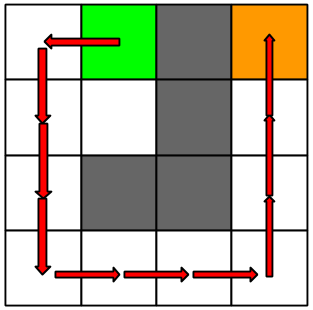
\includegraphics[scale=0.4]{prolog_path}
	\caption{The shortest path from (1,0) to (3,0) is (0,0),(0,1),(0,2),(0,3),(1,3),(2,3),(3,3),(3,2),(3,1),(3,0), 10 steps.}
	\label{path}
\end{figure}
\FloatBarrier


\end{document}
